\documentclass{article}

\usepackage{graphicx}
\usepackage{tikz}
\usepackage{tikzsymbols}
\usetikzlibrary{calc,patterns,shapes.geometric}
\pagestyle{empty}
\usepackage[margin=0pt]{geometry}
\geometry{papersize={14in,12in}}

\def\centerarc[#1](#2)(#3:#4:#5){\draw[#1] ($(#2)+({#5*cos(#3)},{#5*sin(#3)})$) arc (#3:#4:#5);}

\begin{document}
	\begin{figure}
		\centering
		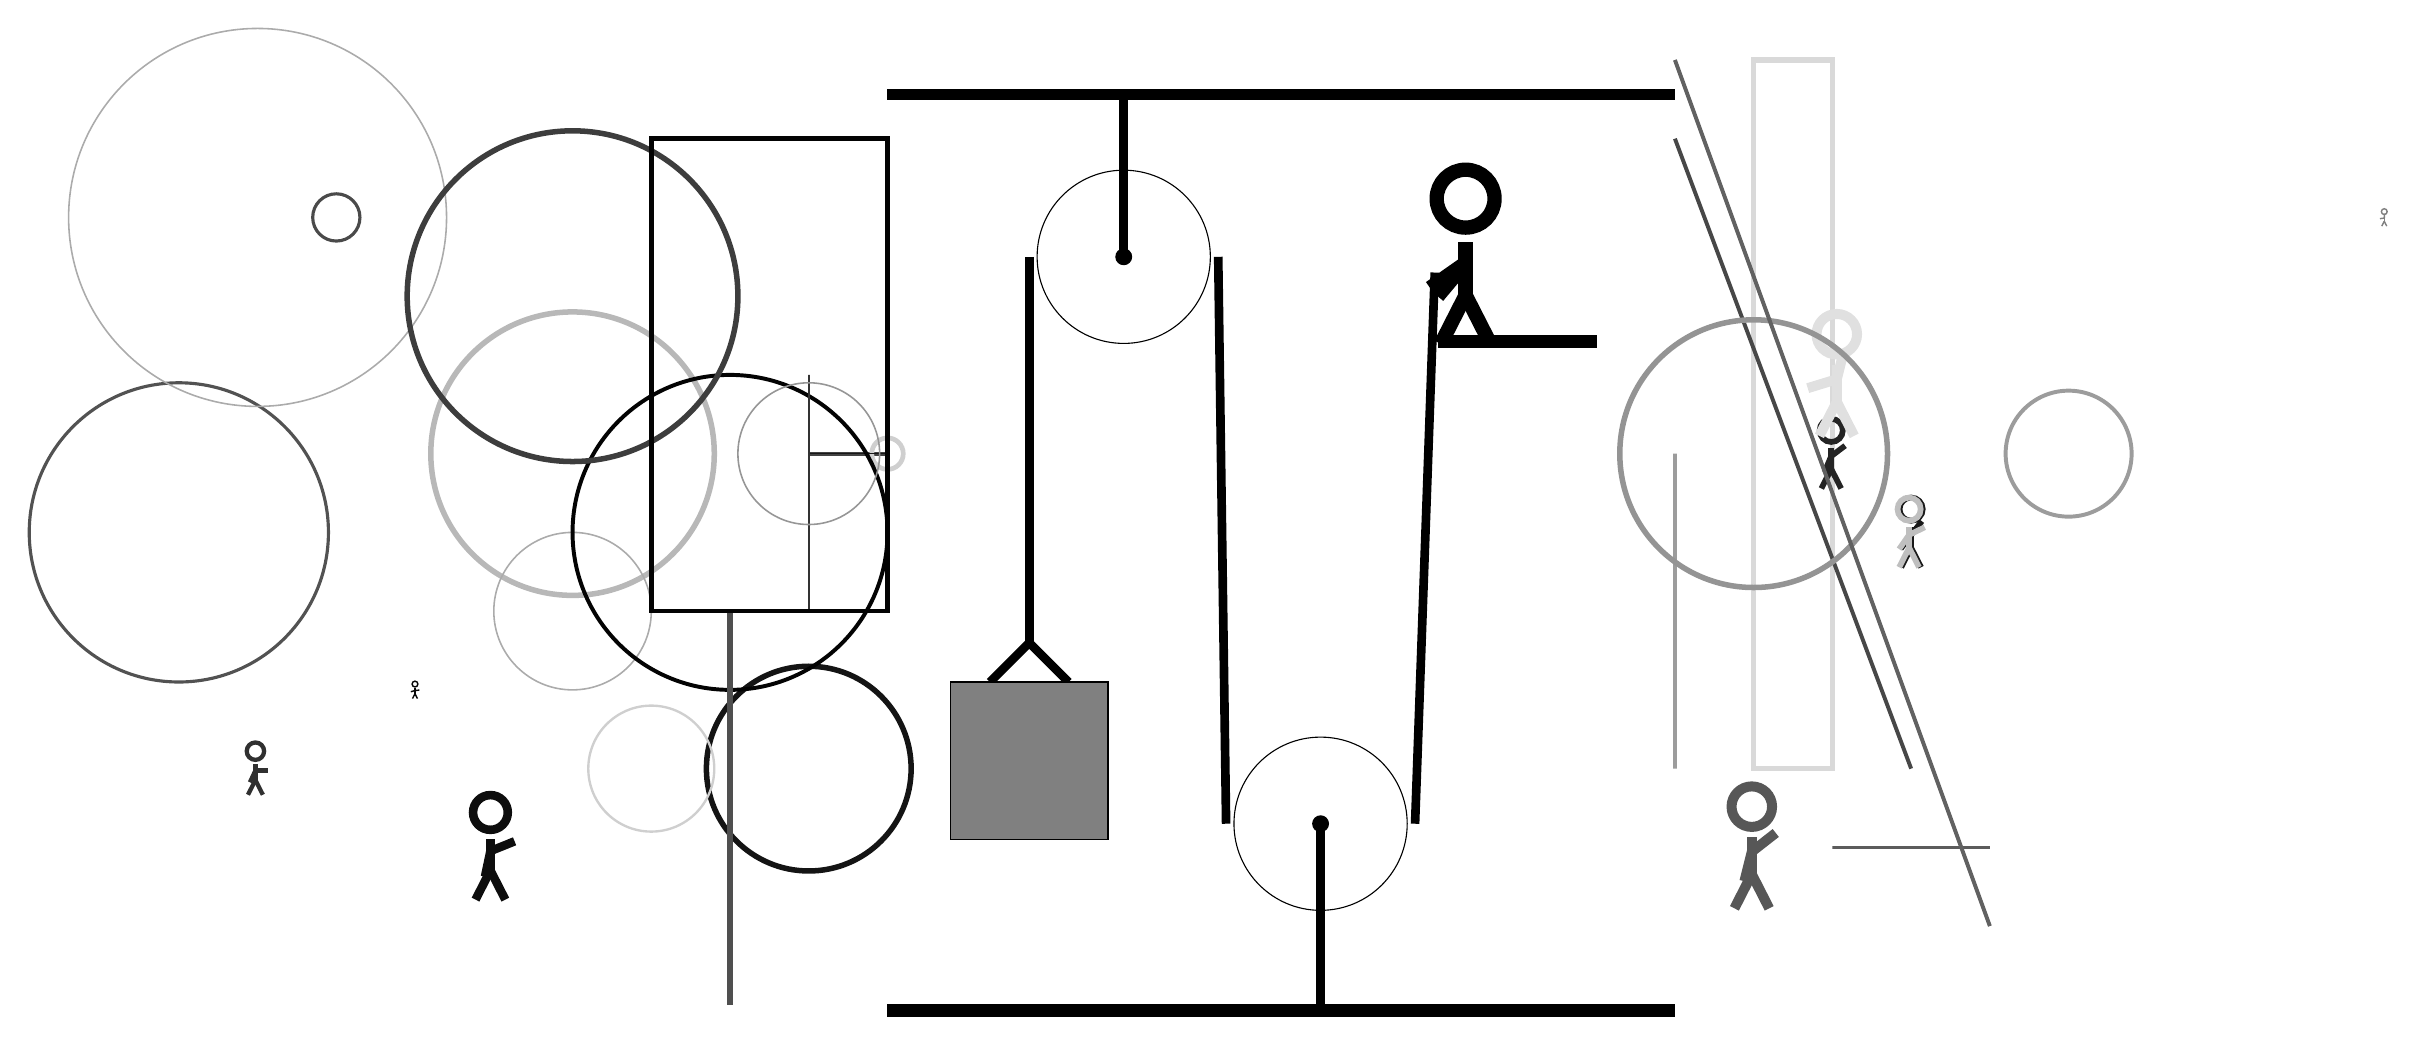
\begin{tikzpicture}
			%%%%% START %%%%%
			
			\draw[fill=black] (-2, 11.5) rectangle (8, 11.625);
			
			\draw (3.5, 2.3) circle (1.1);
			\draw[fill=black] (3.5, 2.3) circle (0.1);
			\draw[line width=1.1mm] (3.5, 2.3) -- (3.5, 0);
			
			\node[line width=0.3mm, color=black!66] at (9, 2) {\Strichmaxerl[7][76][38]};
			
			\draw [line width=0.7mm, color=black!92](-3, 3) circle (1.3);
			\draw [line width=0.5mm, color=black!39](13, 7) circle (0.8);
			\draw [line width=0.7mm, color=black!28](-6, 7) circle (1.8);
			\draw[line width=0.5mm, color=black!74](-3, 7) -- (-2, 7);
			\draw [line width=0.2mm, color=black!33](-6, 5) circle (1.0);
			\draw [line width=0.6mm, color=black!19](-2, 7) circle (0.2);
			\draw[line width=0.7mm, color=black!15] (10, 3) rectangle (9, 12);
			\node[line width=0.7mm, color=black!81] at (-10, 3) {\Strichmaxerl[3][65][0]};
			
			\node[line width=0.2mm, color=black!97] at (-8, 4) {\Strichmaxerl[1][17][5]};
			\draw[line width=0.2mm, color=black!91] (-3, 5) rectangle (-2, 7);
			
			\node[line width=0.3mm, color=black!90] at (11, 6) {\Strichmaxerl[4][53][52]};
			\draw [line width=0.5mm, color=black!99](-4, 6) circle (2.0);
			
			\node[line width=0.3mm, color=black!86] at (10, 7) {\Strichmaxerl[4][67][37]};
			\draw[line width=0.6mm, color=black!39] (8, 7) rectangle (8, 3);
			\draw[line width=0.3mm, color=black!80] (-3, 8) rectangle (-3, 5);
			\draw[line width=0.4mm, color=black!64] (10, 2) rectangle (12, 2);
			\draw [line width=0.4mm, color=black!68](-11, 6) circle (1.9);
			\draw [line width=0.4mm, color=black!71](-9, 10) circle (0.3);
			\draw [line width=0.2mm, color=black!33](-10, 10) circle (2.4);
			\draw[line width=0.7mm, color=black!69] (-4, 5) rectangle (-4, 0);
			
			\draw [line width=0.2mm, color=black!41](-3, 7) circle (0.9);
			\node[line width=0.3mm, color=black!50] at (17, 10) {\Strichmaxerl[1][8][86]};
			\draw[line width=0.5mm, color=black!72](11, 3) -- (8, 11);
			\node[line width=0.4mm, color=black!12] at (10, 8) {\Strichmaxerl[7][17][76]};
			
			\draw [line width=0.7mm, color=black!76](-6, 9) circle (2.1);
			\draw [line width=0.7mm, color=black!42](9, 7) circle (1.7);
			\draw[line width=0.6mm, color=black!99] (-2, 5) rectangle (-5, 11);
			\node[line width=0.3mm, color=black!95] at (-7, 2) {\Strichmaxerl[6][78][22]};
			\draw [line width=0.3mm, color=black!19](-5, 3) circle (0.8);
			\node[line width=0.6mm, color=black!25] at (11, 6) {\Strichmaxerl[4][55][26]};
			\draw[line width=0.5mm, color=black!62](8, 12) -- (12, 1);
			
			\draw (1, 9.5) circle (1.1);
			\draw[fill=black] (1, 9.5) circle (0.1);
			\draw[line width=1.1mm] (1, 11.5) -- (1, 9.5);
			
			\draw[line width=1.1mm](-0.7, 4.1) --  (-0.2, 4.6) -- (0.3, 4.1);
			\draw[fill=black!50] (-1.2, 4.1) rectangle (0.8, 2.1);
			
			\draw[line width=1.1mm](-0.2, 9.5) -- (-0.2, 4.6);
			\centerarc[line width=1.1mm](1, 9.5)(180:0:1.2000000000000002)
			\draw[line width=1.1mm](2.2, 9.5) -- (2.3, 2.3);
			\centerarc[line width=1.1mm](3.5, 2.3)(180:360:1.2000000000000002)
			\draw[line width=1.1mm](4.7, 2.3) -- (4.95, 9.3);
			
			\node at (5.3, 9.5) {\Strichmaxerl[10][35][-130]};
			\draw[fill=black] (5, 8.5) rectangle (7, 8.35);
			
			\draw[fill=black] (-2, 0) rectangle (8, -0.15);
			
			%%%%% END %%%%%
		\end{tikzpicture}
	\end{figure}	
\end{document}